\section{Finite reduction and the canonical atlas}
\label{sec:finite-reduction}

\subsection{Candidate space}

There are $2^{24}-1$ nonempty chamber masks.  A tiler must be connected and
its cardinality must divide $24$.  We first enumerate connected masks, apply
the divisibility filter, and then retain one numeric-minimum representative
from each left $S_4$ orbit.  The reduction is summarised in
\cref{tab:reduction}.

\begin{table}[ht]
\centering
\caption{Exact finite reduction.  ``Eligible'' means connected with chamber
cardinality dividing $24$.}
\label{tab:reduction}
\begin{tabular}{@{}lr@{}}
\toprule
stage & count\\
\midrule
connected nonempty masks & $1{,}210{,}648$\\
eligible connected masks & $67{,}681$\\
canonical eligible left-orbit representatives & $2{,}874$\\
exact left-translate tilers & $97$\\
exact-cover negatives & $2{,}777$\\
convex/nonconvex tiler split & $15/82$\\
\bottomrule
\end{tabular}
\end{table}

\begin{lemma}[Canonical reduction]\label[lemma]{lem:canonical-reduction}
Every connected piece is left-equivalent to exactly one stored canonical
mask.  A canonical piece is a left-translate tiler if and only if the
exact-cover recursion below returns a cover.
\end{lemma}
\begin{proof}
The finite orbit $\{gU:g\in S_4\}$ has a unique minimum integer mask.  Left
multiplication preserves adjacency by \cref{lem:basic-covariance}.  Every
cover of any orbit member translates to a cover of the canonical member, and
conversely.  It therefore remains only to show that the recursion enumerates
all covers, which is \cref{lem:exact-cover-completeness} below.
\end{proof}

\subsection{Exact-cover search}

For a fixed canonical $U$, let $\mathcal O$ be the set of distinct masks in
$\Orb_L(U)$.  A search state is a pair $(R,\mathcal F)$, where $R$ is the
remaining uncovered mask and $\mathcal F$ is the chosen family.  Initially
$R=G$ and $\mathcal F=\varnothing$.  At a nonterminal state choose the
least-indexed chamber $c$ of $R$ and branch over all $V\in\mathcal O$ with
$c\in V\subseteq R$.

\begin{algorithm}[Least-uncovered exact-cover recursion]
\label[algorithm]{alg:exact-cover}
\begin{enumerate}[leftmargin=2.2em]
\item If $R=\varnothing$, output $\mathcal F$.
\item Let $c$ be the least chamber contained in $R$.
\item For every $V\in\mathcal O$ with $c\in V$ and $V\cap(G\setminus R)
=\varnothing$, recurse on $(R\setminus V,\mathcal F\cup\{V\})$.
\end{enumerate}
\end{algorithm}

\begin{lemma}[Exact-cover completeness]\label[lemma]{lem:exact-cover-completeness}
\Cref{alg:exact-cover} outputs every unordered exact cover of $G$ by members
of $\Orb_L(U)$ exactly once.
\end{lemma}
\begin{proof}
Let $\C$ be an exact cover extending the current partial family.  The least
uncovered chamber $c$ belongs to a unique member $V$ of $\C$.  That member is
one of the algorithm's branches, so induction on the number of uncovered
chambers reaches $\C$.  Conversely, each branch adds a subset of the remaining
mask, hence every terminal family is disjoint and covers $G$.  Choosing the
least uncovered chamber makes the sequence of chosen members canonical for
an unordered cover, so no cover is output twice.
\end{proof}

Two independent implementations support the enumeration.  The source-replay
lane executes the earlier T2 algorithms at their pinned revision.  The
independent lane scans all nonempty $24$-bit masks, reconstructs the chamber
graph, halfspace closure, orbit canonicalisation, and exact-cover recursion
without importing the T2 code.  The two lanes agree on the entire $97$-row
positive stream and its exact digest.

\subsection{The atlas theorem}

\begin{theorem}[Canonical nonconvex left-translate atlas]
\label{thm:left-atlas}
Up to left $S_4$ equivalence, exactly $82$ connected
halfspace-nonconvex pieces tile the reference tetrahedron by left translates.
Their distribution is
\[
\begin{array}{c|ccc}
|U|&6&8&12\\ \hline
\#\text{ orbits}&14&18&50.
\end{array}
\]
Together with the $15$ convex types of \cite{BabanskyyT2}, they exhaust the
$97$ positive canonical representatives in \cref{tab:reduction}.
\end{theorem}
\begin{proof}
By \cref{lem:canonical-reduction,lem:exact-cover-completeness}, the exhaustive
candidate scan and exact-cover recursion decide every eligible left orbit.
Both implementations find the same $2{,}777$ negatives and $97$ positives.
The halfspace predicate, calibrated against the imported three-way convexity
theorem on connected masks, divides the positives into $15$ convex and $82$
nonconvex rows.  Grouping the latter by popcount gives $14,18,50$.
\end{proof}

\begin{figure}[ht]
\centering
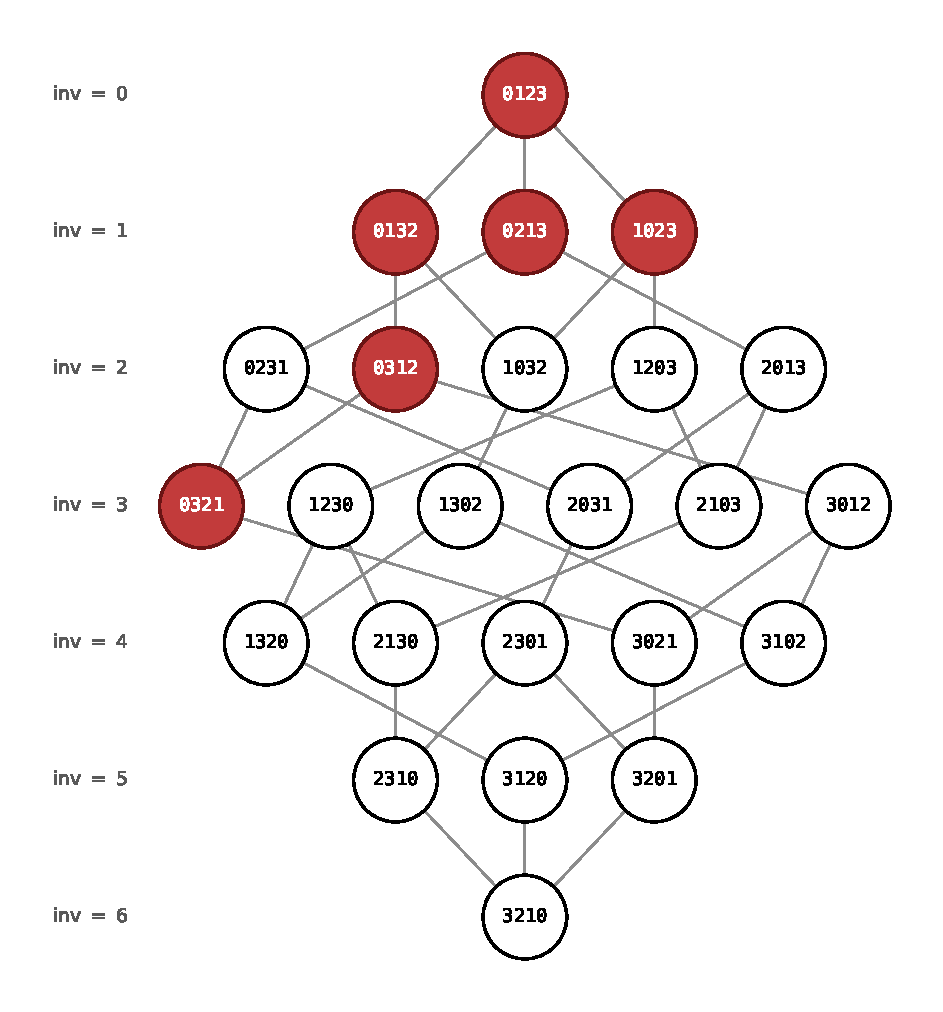
\includegraphics[width=.72\textwidth]{figures/t2_nonconvex_example.pdf}
\caption{The chamber set of the six-chamber row
\rowid{P18-NC-K06-M000077}, highlighted in the $A_3$ chamber graph.  This
was the existence witness used to show that the nonconvex problem is
nonempty in \cite{BabanskyyT2}; here it is one row of the complete atlas.
Figure reused under CC BY 4.0.}
\label{fig:nonconvex-example}
\end{figure}

Every atlas row has the content-addressed identifier
\[
 \rowid{P18-NC-K}\,|U|\,\rowid{-M}\,m(U),
\]
with the cardinality written in two decimal digits and the mask in six
uppercase hexadecimal digits.  For example, the first row is
\rowid{P18-NC-K06-M00006F}.  Source-array positions are locators, never row
identity.  The complete table appears in \cref{app:catalogue}.

\subsection{Congruence closure of the candidate universe}
\label{sec:congruence-closure}

The left-translate census is only the combinatorial half of the earlier
congruent-copy problem.  The missing implication is global: a
left-exact-cover negative must not become positive by using congruent
Coxeter-pure pieces drawn from several left orbits.  It would be circular to
check this only on the $82$ already selected rows.

The ambient argument in \cref{sec:ambient} therefore runs on all $2{,}874$
eligible canonical candidates.  \Cref{thm:global-rigidity} proves that free
Euclidean congruence equals left $S_4$ equivalence throughout that carrier,
and \cref{cor:congruent-atlas} promotes \cref{thm:left-atlas} to the complete
classification by congruent Coxeter-pure copies.  No equivalence is assumed
in the exact-cover search itself.
